\chapter{系统设计与实现}

\section{系统设计目标}

针对“三高”慢性病医学问答场景中专业信息较多、回答可靠性要求较高、交互反馈也比较明显的特点，本文设计并实现了一套基于检索增强生成的智能医学问答系统，并结合医学问答任务本身的需求，提出了四个方面的系统设计目标。

一是准确性，医学问答系统首先要尽量保证回答内容科学、准确，因为医学知识本身专业性很强，一旦出现错误或表述不严谨，就可能误导用户，甚至带来潜在风险。为了解决这个问题，系统构建了较高质量的“三高”慢性病医学知识库，并采用关键词检索和语义向量检索结合的混合检索策略，从权威资料中找出和用户问题高度相关的医学证据，再借助RAG机制把这些证据送入大语言模型作为回答依据，从而减少模型凭空编造内容的情况，提高回答的事实一致性和专业可靠性。

二是可解释性，和通用问答系统相比，医学问答不只是给出结论，还要让使用者看清结论依据来自哪里。基于这一点，系统在生成回答时，会同时保留并展示相关医学证据的来源信息，比如指南、科普文章或其他参考资料，通过“回答正文加引用来源”的形式，让结论来源能够被进一步追溯；同时，系统也会在提示词设计中对模型输出加入结构化约束，引导生成内容尽量围绕检索到的证据展开，从而进一步增强结果的可解释性。

三是实时性，在实际使用过程中，用户通常希望较快得到问答结果，因此系统需要具备较好的响应速度。考虑到大语言模型推理本身计算开销较大，系统将模型部署在高性能服务器上，并加入多种性能优化方式，包括利用向量检索加快知识匹配过程、使用混合精度计算降低推理开销，以及通过键值缓存减少重复计算，从而提升整体生成效率；在系统架构上，系统还采用前后端分离设计，使用户请求能够更快完成处理和返回，以满足实时交互的需要。

四是可扩展性，医学知识会不断更新，应用需求也会持续变化，因此系统还需要保留较好的扩展能力。一方面，知识库采用模块化管理方式，支持医学数据的新增、修改和维护，便于后续持续纳入新的医学指南和研究成果；另一方面，系统在架构设计上让知识库、检索模块和生成模型之间保持相对松耦合的关系，使各部分能够独立升级或替换，比如可以在不影响整体结构的情况下更换性能更好的向量模型或大语言模型，这样也能为系统后续的演进和适应能力留出足够空间。

\section{系统总体架构}

本系统整体架构采用分层式设计，将交互逻辑、业务逻辑、模型能力与数据能力进行划分，各模块之间相对独立，能够在一定程度上实现故障隔离。系统架构如图4.1所示，主要由四个层次构成。

前端应用层只承担交互和状态管理，不直接参与模型推理，具体包括用户登录、会话管理、消息渲染、流式展示、引用证据呈现以及管理员知识库入口等功能。

业务服务层基于Node.js，采用Express框架构建统一的 API 网关，用于对外提供服务接口。业务服务层主要负责身份认证与权限控制、会话上下文组织、消息持久化、模型服务编排和知识库维护。

模型推理层是一套独立的Python服务，部署在高性能GPU服务器上，基于Flask框架对外提供接口。该层主要负责向量数据库检索、相关文档重排序、提示词组装、模型推理及流式事件输出。模型服务对外暴露同步与流式两类接口，业务服务可以根据实际场景灵活选择调用方式。将推理服务独立部署后，可在不影响业务API的情况下单独升级模型和检索策略。

数据与索引层中使用关系型数据库保存用户、会话、消息与文档元数据；使用FAISS向量索引存储医学指南等医学资料，并将文本编码为向量构建索引结构以支持向量检索和BM25检索。

\vspace{10pt}
\begin{figure}[htb]
    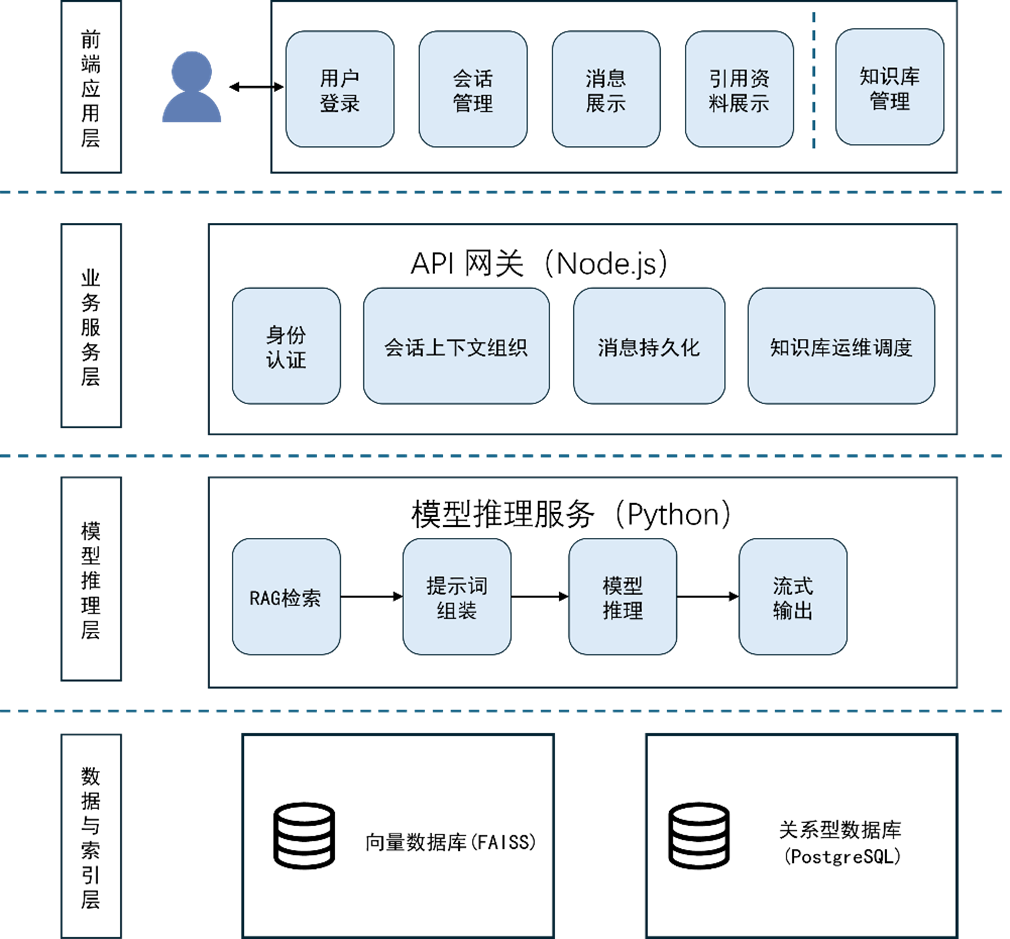
\includegraphics[width=0.7 \textwidth]{image/4/系统架构图.png}
    \caption{系统架构图}
    \label{fig:framework-structure}
\end{figure}

\section{系统流程设计}

在输入解析阶段，系统会先接收用户发来的自然语言问句，再结合之前几轮对话的历史信息对查询做语义补全和规范化处理，从而让后续检索能更精准地锁定用户真正的意图。

在知识检索阶段，系统采用混合检索策略，一路是基于向量的语义检索，它依靠Embedding模型把文本映射到高维的向量空间中来表示语义、捕捉深层的语义相似性；另一路则是基于关键词的BM25检索，专门负责精确锁定关键字上的匹配，特别针对于医学领域海量的专业术语。如果只依赖向量检索，有可能会漏掉或误判某些关键医学名词，于是把BM25作为补充手段能有效提高整个检索结果的准确度和覆盖面，两路结果检索完成之后，系统再经过融合、排序和重排这几道处理，筛选出最相关的一批文本片段。

在上下文增强阶段，系统将上一阶段筛选出的文本片段，用户问题和对话历史，通过事先设计好的prompt模板结合，构建成一份结构清晰的输入，让模型在阅读时能轻易分辨出哪一部分来自使用者的提问、哪一部分是从知识库里调出来的参考资料。

在答案生成阶段，模型依据这份组合好的输入来产出回答，以流式方式逐字输出。在生成全部完成后，系统会把检索到的文献信息返还给用户当成参考，同时也会记录下这次输入和输出所消耗的token数量，后者将会跟对话历史一同保存进数据库，为下一次用户提问时构建多轮对话上下文时估算长度提供依据。

\section{业务层实现}

业务层后端服务基于Node.js的框架Express开发，负责用户身份认证与权限控制、会话管理、消息持久化、模型服务编排与知识库运维接口。

\subsection{后端服务架构设计}

系统后端入口位于统一应用服务中，主要路由模块包括用户认证、会话管理、消息管理、模型调用和知识库管理。各模块职责如下：
\begin{enumerate}[label =(\arabic*)]

    \item 认证模块：提供注册与登录接口，完成密码加密与令牌签发；
    \item 会话模块：管理会话创建、查询、更新与软删除；
    \item 消息模块：管理消息读写与 token 信息回填；
    \item 模型模块：接收问题请求，调用本地模型服务并返回生成结果；
    \item 知识库模块：提供文档元信息管理、索引状态查询与重建能力。

\end{enumerate}

\subsection{会话管理}

会话管理是后端业务逻辑中的核心部分。系统为每个用户维护独立会话空间，并将每轮对话中的角色、正文、时间戳、引用证据和统计信息写入数据库，以支撑历史记录查询和多轮上下文组织。

在具体流程上，当用户提交问题时，后端会先判断当前会话是否存在；若不存在，则创建新会话并写入用户消息；若已存在，则直接在原会话下追加消息。模型返回回答后，系统再将助手回答与证据一并写回，并同步更新会话摘要和更新时间。这样既能保证多轮对话连续性，也方便前端展示最近会话状态。

\subsection{数据库}

后端数据库使用PostgreSQL，PostgreSQL可支持使用“JSONB内容字段”的存储。在保存用户与模型的对话历史时，用户消息和模型消息、系统消息的结构并不完全相同，例如：模型消息在返回时会携带RAG过程中检索到的资料信息，而用户消息则不需要这个字段。面对这类字段需求参差不齐的情况，JSONB 格式比常规的关系型表设计要灵活得多，能很好地应对问答消息里字段不固定、结构可能时常变动的状况。系统将用户、会话、消息等较为固定的实体信息保存在关系型字段里；将消息正文、引用资料信息、Token消耗等可选字段的内容存放在JSONB字段中。通过这一混合存储方式，就能用同一张表适应模型消息和用户消息的不同格式，不必再去为每一种消息单独建表。 

表4.1中列出了系统中关键的数据表及其主要字段，其中，users表用于存储用户信息，并且为每个用户分配独特的id，用户id是对其他表查询的关键信息；conversations表用于存储会话元信息（标题、更新时间、软删除标记等）；messages表用于保存逐轮对话内容与token统计信息；medical\_documents表用于保存知识文档元数据；knowledge\_index\_meta表用于记录索引状态（dirty/running/synced/error）。

\begin{table}[htbp]
    \centering
    \caption{后端核心数据表}
    
    \setlength{\tabcolsep}{8pt} % 列间距（原来14mm太大了）
    
    \begin{tabular}{l c p{5cm}} % 第三列自动换行
        \toprule
        数据表名 & 核心字段 & 作用 \\
        \midrule
        user & id, password\_hash, is\_admin & 用户身份与权限管理 \\
        conversations & user\_id, title, last\_message, is\_deleted & 会话元信息管理 \\
        messages & conversation\_id, role, content, tokens & 多轮消息与 token 信息存储 \\
        medical\_documents  &  title, source, ingest\_key, tags &  知识文档元信息维护 \\
        knowledge\_index\_meta  &  status, last\_reindexed\_at, last\_error  &  索引状态追踪与运维监控 \\
        \bottomrule
    \end{tabular}
\end{table}

\subsection{流式转发}

为了缩短用户等待时的空白感，后端加入了面向前端的流式转发机制，Node.js服务接收到模型服务返回的增量文本后，会继续通过SSE把内容持续发送到前端，这样回答还没有完全生成时，界面上就已经能看到文本逐步显示出来，整体交互会更连贯。

具体处理时，后端会先把用户消息和助手占位消息写入数据库，再和模型服务建立流式连接，后续只要模型服务持续返回新的文本片段，后端就会把这些内容整理成前端可以解析的事件数据并立即转发出去；等回答生成结束后，再统一回写完整结果和相关统计信息，这样一来，界面能够及时更新，数据库里保存的内容也能保持完整一致。

\subsection{知识库管理接口}

知识库管理接口主要面向管理员使用，任务是把文档维护和索引管理这一类后台操作组织起来，接口内容包括文档元信息查询、文本上传入库、索引状态查看、增量更新和全量重建等，这样知识库相关操作就能放在统一入口中处理，管理起来也更方便。

在知识入库过程中，后端接收到文本内容和来源信息后，会继续调用后续处理流程，依次完成文本清洗、内容切分、Embedding编码和索引写入，写入成功以后，再触发模型服务对索引进行热更新；如果中间某个环节出现问题，系统会把错误状态记录下来，并返回较明确的提示信息，方便后面排查和恢复，这样处理之后，知识更新就不再是彼此分散的单独步骤，而是能和在线问答过程更自然地衔接起来。

\section{模型服务实现}

\subsection{Qwen推理服务}

模型服务采用Python独立实现，其中Qwen推理模块负责最终回答生成。系统启动时加载基础模型和分词器，并根据资源条件选择相应推理方式。问答过程中，模型服务接收后端转发的问题、上下文和参数配置，将其组织为统一输入后交给Qwen模型执行生成。

选择Qwen作为生成核心，主要考虑其中文能力较强，且能够较好处理长上下文和说明性回答。与RAG和DPO模块结合后，Qwen不仅承担“生成文本”的任务，也成为系统将检索证据转化为自然语言答复的关键执行单元。

\subsection{bge Embedding服务}

为支持语义检索，模型服务内部集成bge Embedding模型，对用户查询和知识文本进行向量化表示。知识入库阶段，系统对文本块编码并写入向量索引；在线问答阶段，再对用户问题执行同样的编码操作，以完成相似度检索。

Embedding服务的价值在于，它让系统能够理解不同表述之间的语义接近关系，而不必拘泥于字面一致。对于大量口语化、症状化的慢病咨询问题，这一点尤为重要。

\subsection{DPO模型加载与推理}

除基础Qwen模型外，系统还支持加载经DPO训练得到的适配权重，以进一步优化医学场景下的回答偏好。部署时，这部分权重通常以适配器形式保存，模型服务按配置完成加载，并与基础模型共同组成最终推理模型。

在实际推理中，DPO优化不会改变检索结果本身，但会影响模型如何组织回答。例如，当问题涉及治疗建议、用药风险或证据不足时，模型会更倾向于采用审慎表述，并主动提醒线下就医或补充信息。这种变化正是偏好优化在医学场景中的主要价值。

\subsection{流式输出}

模型服务同时支持同步生成和流式生成两种模式。流式模式下，服务会持续返回模型生成的文本片段，使回答具备边生成边展示的效果，从而明显改善交互体验。

在实现上，模型服务通过SSE事件格式向后端发送\texttt{delta}、\texttt{end}和\texttt{error}等事件；后端再将这些事件继续转发到前端，形成端到端的流式问答链路。这一设计让系统既能保持低时延反馈，也能在异常情况下提供较清晰的错误处理路径。

\section{RAG服务工程实现}

\subsection{检索调用流程}

在RAG服务运行时，模型服务首先接收用户问题，并结合必要的历史对话构造检索查询。随后，系统并行调用BM25和向量检索，分别得到关键词相关候选和语义相关候选，形成双路初召回结果。

完成召回后，系统对候选文本进行统一标识、合并与去重，再进入融合排序和重排阶段。最终保留下来的高质量证据会被组织为结构化上下文，并传递给生成模块。整个流程强调的是“先保证不漏，再尽量选准”。

\subsection{BM25 + 向量融合实现}

在工程实现上，BM25和向量检索保持相对独立的召回路径，系统在候选层面对两类结果进行统一融合。BM25负责抓住关键术语，向量检索负责补足语义改写，两者组合后能够更稳妥地应对真实问答中的表达差异。

融合时，系统根据候选在不同检索列表中的相对位置综合计算优先级，使在多路检索中都表现靠前的文本获得更高排序。这样做避免了单一路径偏差对最终结果造成过大影响。

\subsection{Rerank实现}

融合后的候选结果仍可能包含主题相关但并不适合直接作答的文本，因此系统进一步引入重排模型进行精筛。与初召回不同，重排阶段更关注“这段文本是否最适合回答当前问题”，而不是“它是否大致相关”。

在实现中，系统逐条计算候选证据与问题之间的匹配程度，并据此重新排序，再从中选出Top-$K$文本作为最终证据。该步骤能够明显降低噪声片段进入生成阶段的概率，是提升回答质量的重要环节。

\subsection{上下文拼接}

在获得最终证据后，系统需要将其组织成模型可直接利用的输入上下文。拼接时，系统会保留证据来源、标题和正文片段，并按相关性顺序写入Prompt中，使模型既能看到内容本身，也能感知其来源背景。

同时，系统会控制证据条数和单条长度，避免长文本挤占过多上下文空间。对于多轮问答，还会加入必要的近期历史消息，以帮助模型更准确地理解当前问题与前文之间的关系。

\section{前端实现}

\subsection{前端UI架构与路由设计}

前端界面采用React构建，并结合路由机制完成页面切换，整体上分为登录页、注册页、问答主页和知识库管理页，不同页面各自承担明确任务，这样既方便功能拆分，也有利于后续继续补充新模块。登录和注册页面主要处理身份验证，问答主页负责会话列表、消息展示和问题输入，知识库管理页则面向管理员，用来处理文档维护与索引相关操作。

在界面组织上，前端把通用能力拆分到页面、组件和Hook三个层次，页面负责整体布局和功能组合，组件负责消息列表、输入框、侧边栏等可复用界面，Hook负责会话状态、消息请求和交互流程管理，这种划分方式能让界面结构更清楚，代码之间的联系也更容易梳理。主页部分采用侧边栏与主内容区的布局，侧边栏用于展示历史会话和常用操作，主区域用于展示问答内容与输入区域，页面层次比较直观，用户进入系统后也能较快找到对应功能。

\subsection{对话交互与流式渲染实现}

会话相关的核心逻辑集中放在自定义Hook中，发送问题时，界面会先把用户消息和助手的占位内容加入当前会话，再向后端发起流式请求，这样用户提交问题后能马上看到界面变化，等待过程也不会显得突兀。流式数据通过后端的SSE通道持续返回，前端再用ReadableStream按帧读取并解析事件，接收到\texttt{delta}内容后，就把新增文本接到助手回答后面，于是回答会一点点展开，形成较自然的实时反馈效果。

为了让多轮对话前后保持一致，流式输出结束后，前端还会重新拉取一次消息记录，并用后端已经保存的结果覆盖临时状态，避免在长对话过程中因为局部丢帧或上下文偏移，出现界面显示和实际数据不一致的情况；如果模型服务中途异常或连接中断，界面会直接给出明确的提示文本，使当前交互还能继续恢复，不会停在难以理解的状态里。

\subsection{消息展示与检索证据可视化}

消息展示部分支持Markdown和GFM语法渲染，因此回答中的分点说明、表格以及部分结构化内容都能较完整地显示出来，页面阅读体验也更清楚。在RAG问答场景下，系统会把检索得到的\texttt{retrieved\_docs}附加到助手消息中，再在回答下方用“全部引用”的折叠区域统一展示，这样答案和证据能够放在同一界面里，用户查看结论时也能顺带看到对应依据，有助于增强结果的可解释性与可追溯性。

为了减少重复信息，前端会按照\texttt{source}字段对引用文档进行去重，同时保留来源名称、标题层级等关键内容，便于快速核对回答依据，也便于进一步判断相关结论是否来自较可靠的医学资料，从而提高对系统输出结果的信任程度。

\section{本章小结}

本章从工程实现角度介绍了医学问答系统的整体设计。首先明确了系统在准确性、可解释性、实时性和可扩展性方面的目标；随后说明了总体架构和RAG运行流程；最后分别从后端、模型服务、RAG工程实现和前端交互四个层面展开具体实现分析。

通过上述设计与实现，本文完成了一套具备知识检索、模型生成、证据展示和会话管理能力的医学问答系统，为后续实验评估和应用验证提供了完整工程基础。
